\section{Results}
This chapter presents the results obtained from the Monte Carlo simulations. First, a representative spin configuration containing skyrmionic structures is examined. The corresponding discretized topological charge density is then calculated and used to demonstrate the skyrmion detection procedure developed in this work.

After validating the detection method, the external magnetic field and Dzyaloshinskii--Moriya (DM) interaction strength are varied to construct phase diagrams of the system. These phase diagrams are used to identify the regions corresponding to ferromagnetic, spiral, and skyrmionic phases. Finally, the evolution of the skyrmionic phase with temperature is investigated. This is done by quenching the system at different temperatures, and destroying formed skyrmions by increasing the temperature.


\subsection{Spin lattice}

A $(40\times40)$ spin lattice was initialized with random spin orientations and evolved using the Monte Carlo algorithm described previously. The simulation was first performed at a high dimensionless temperature to ensure thermalization. The temperature was then gradually reduced until the desired value was reached. Figure~\ref{fig: Energy time} shows the evolution of the energy during this process. At each temperature step the energy rapidly approaches a stable value, indicating that the system has reached thermal equilibrium before the temperature is reduced further.

\begin{figure}[H]
	\centering
	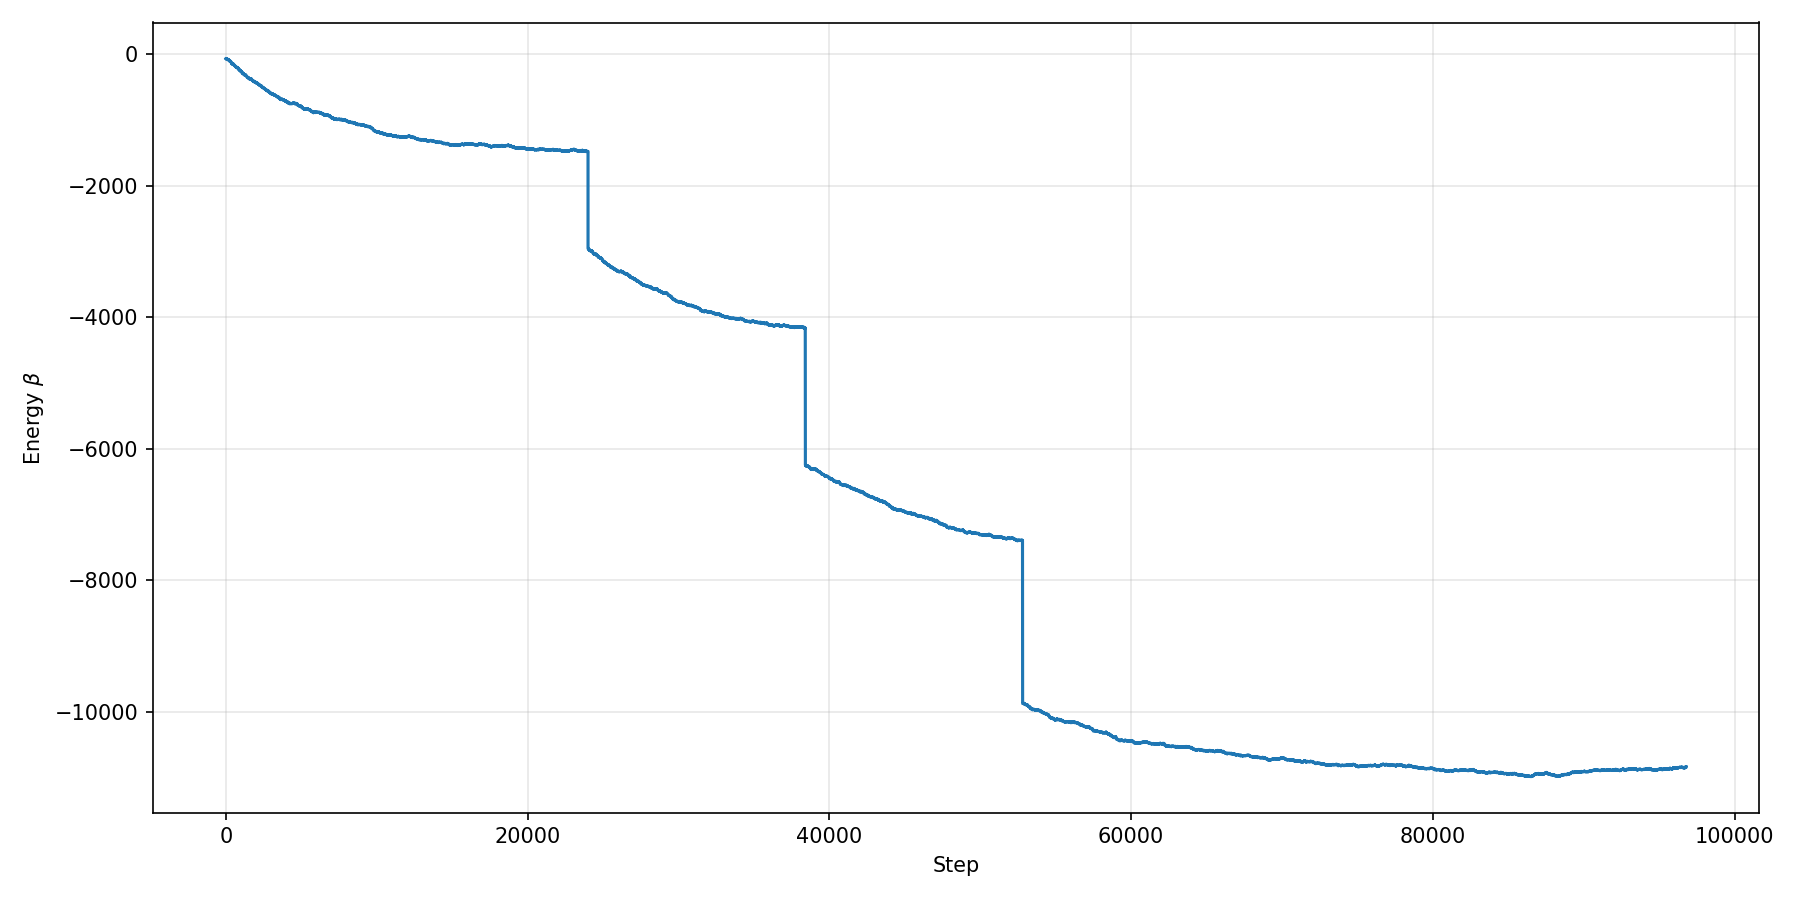
\includegraphics[width = \linewidth]{sections/Graphs/energybeta_evolution.png}
	\caption{The energy as a function of MC steps, showing where the unitless temperature is changed.}
	\label{fig: Energy time}
\end{figure}

Once the final temperature had been reached and the energy had stabilized, spin configurations were sampled from the simulation. An example of such a spin configuration is shown in Figure~\ref{fig: lattice}.

\begin{figure}[H]
	\centering
	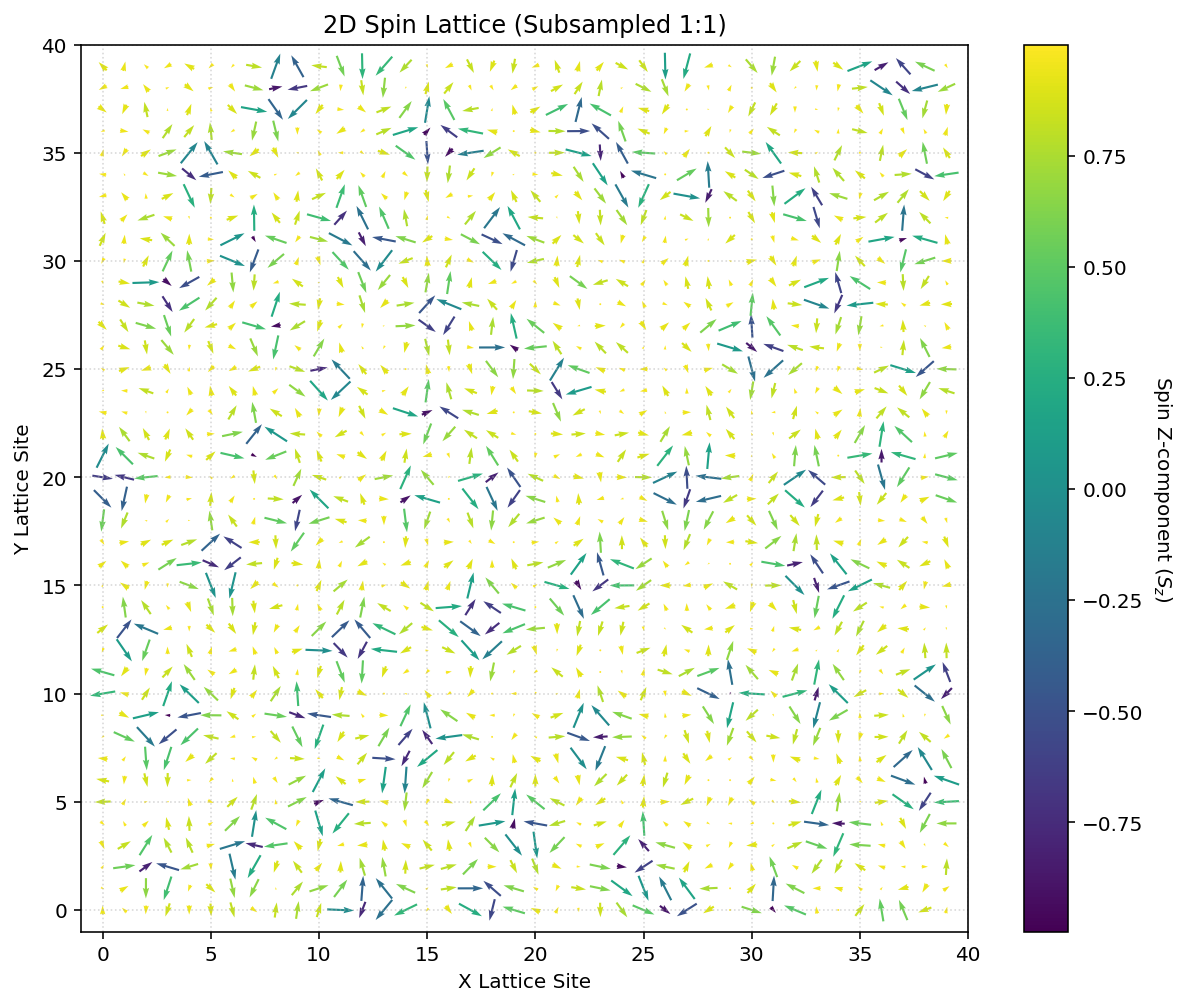
\includegraphics[width = \linewidth]{sections/Graphs/Lattice.png}
	\caption{An example of the spin lattice}
	\label{fig: lattice}
\end{figure}

For each sampled spin lattice, the discretized topological charge density was calculated using the procedure described in Section \ref{model_skyrmion_number}. An example of the resulting topological charge density is shown in Figure~\ref{fig: wrapping}. Regions with a large negative topological charge density correspond to the cores of skyrmionic structures.

\begin{figure}[H]
	\centering
	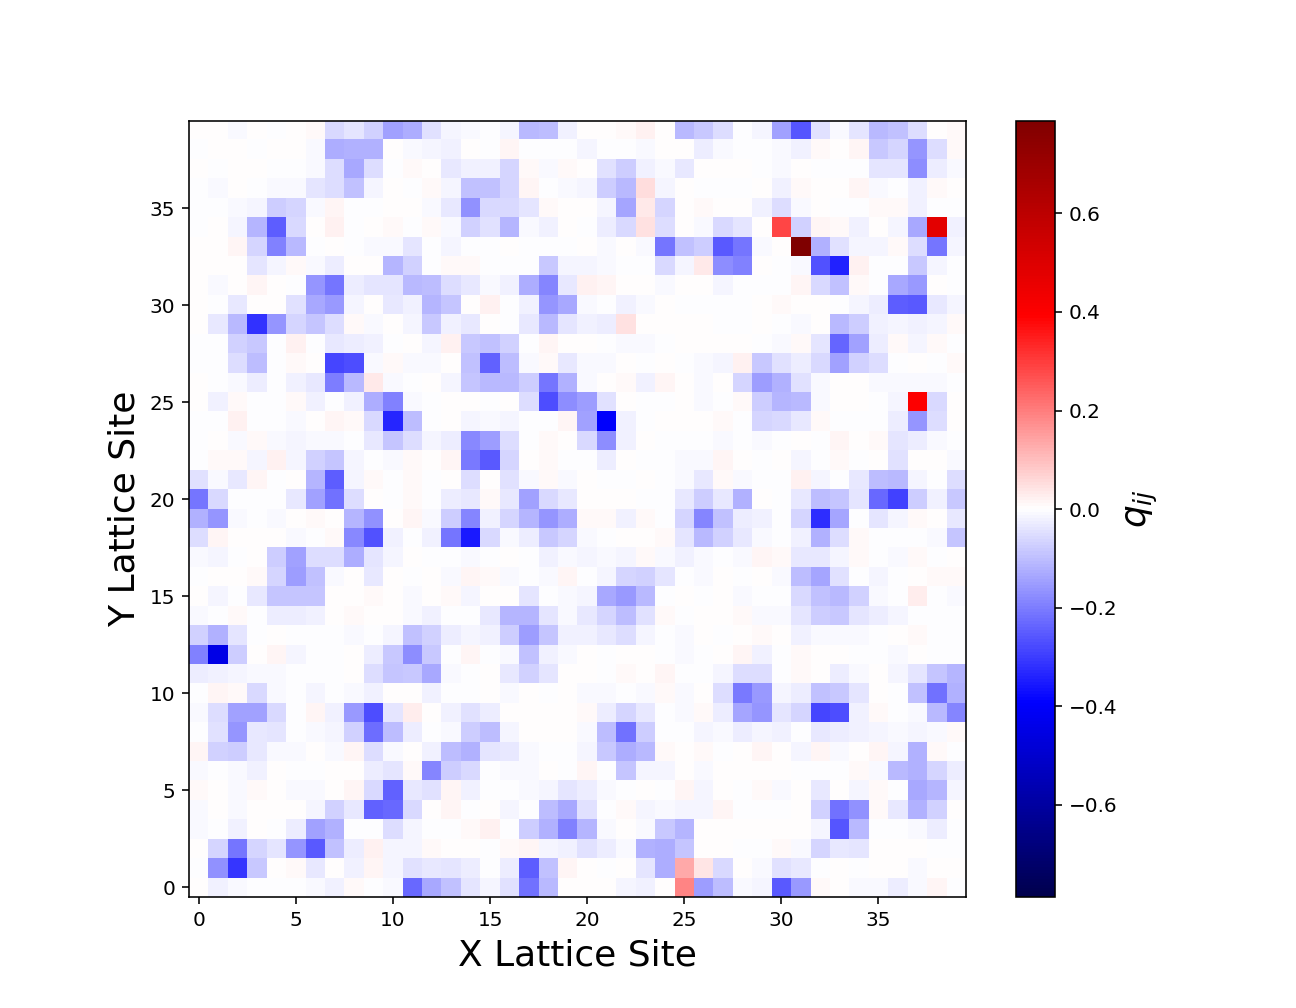
\includegraphics[width = \linewidth]{sections/Graphs/wrapping.png}
	\caption{An example of the winding number calculated from the spin lattice}
	\label{fig: wrapping}
\end{figure}


\subsection{Finding skyrmions}

Skyrmions are characterized by a localized topological charge density. To identify these structures, the calculated topological charge density is first smoothed using a Gaussian convolution in order to suppress thermal fluctuations. An example of the smoothed topological charge density is shown in Figure~\ref{fig: smooth}.

\begin{figure}[H]
	\centering
	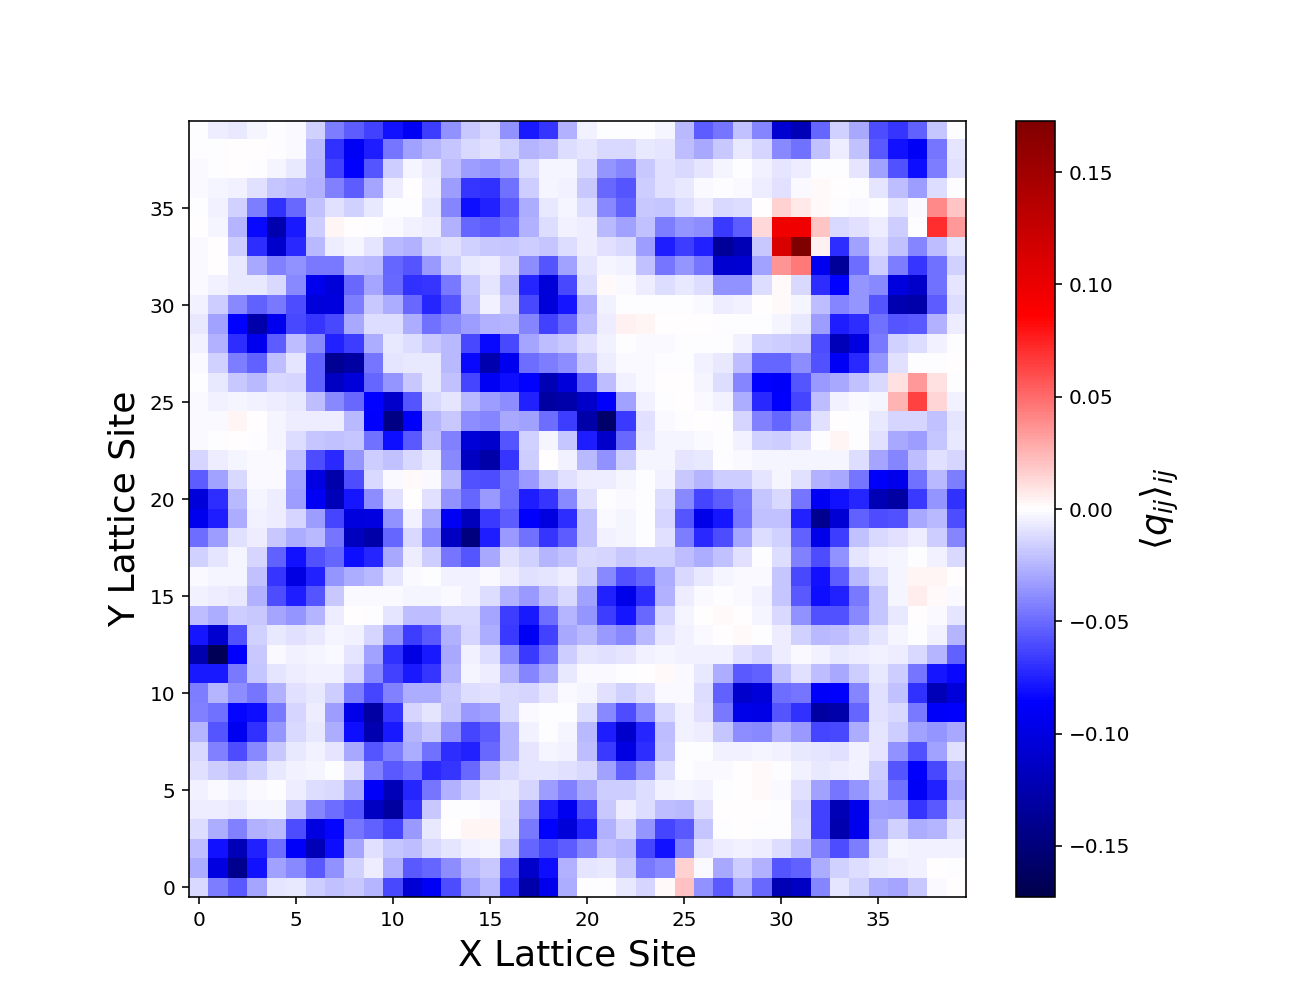
\includegraphics[width = \linewidth]{sections/Graphs/smoothed.png}
	\caption{An example of the winding number calculated from the spin lattice with a Gaussian smoothing.}
	\label{fig: smooth}
\end{figure}

In the smoothed distribution, positive skyrmions correspond to localized positive peaks, while negative skyrmions correspond to localized negative peaks. Candidate skyrmion positions are identified by searching for local maxima and minima. An example of the detected extrema is shown in Figure~\ref{fig: max min}.

\begin{figure}[H]
	\centering
	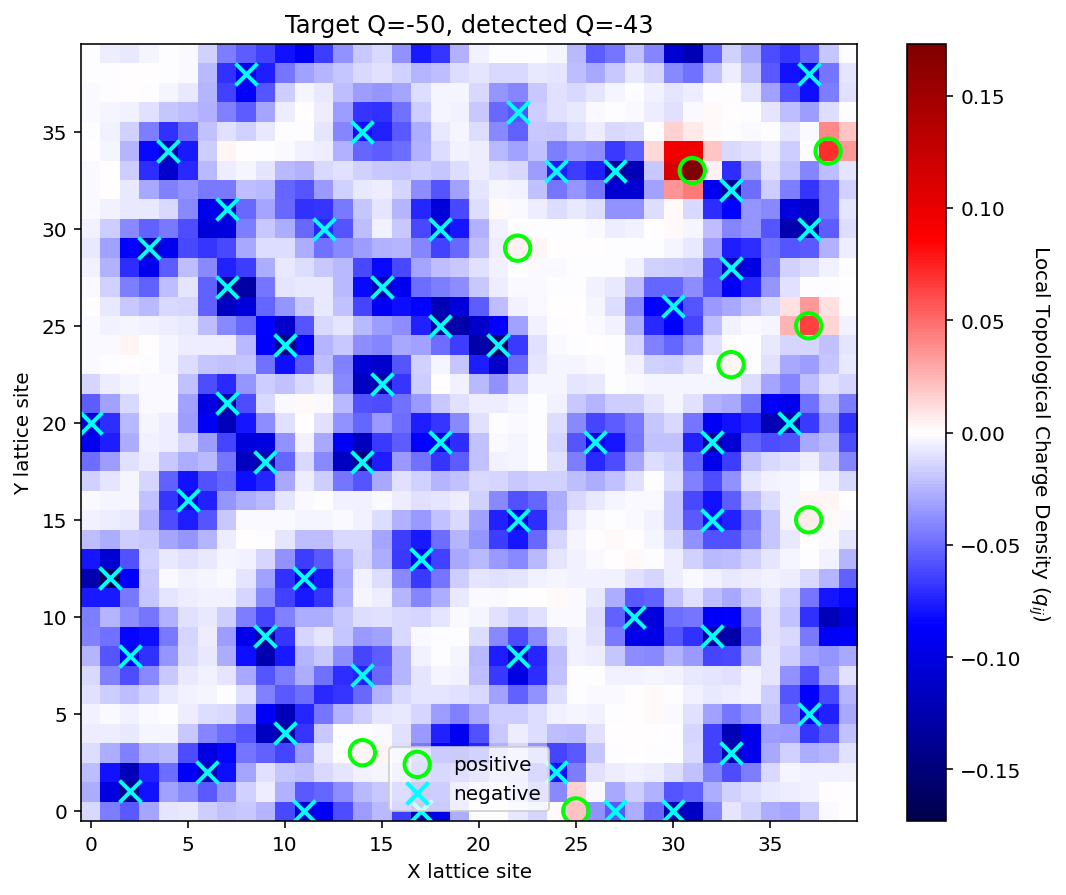
\includegraphics[width = \linewidth]{sections/Graphs/detection.png}
	\caption{An example of the smoothed winding number with the detected minima and maxima (skyrmions).}
	\label{fig: max min}
\end{figure}

Not every detected extremum corresponds to a skyrmion, as thermal fluctuations can also produce local peaks. To distinguish genuine skyrmions from fluctuations, the total topological charge is calculated by summing the local topological charge density over the entire lattice. The resulting integer-valued topological charge provides the net number of positive and negative skyrmions present in the system.

The detected extrema are then ranked according to their magnitude. Starting from the strongest extrema, peaks are successively included until the number of detected structures is consistent with the total topological charge (Q). In this way, weak extrema originating from thermal fluctuations are excluded, while the physically relevant skyrmionic structures are retained.






%\subsection{Distinguishing phases}
%
%there are a few phases to be found here, one where the ferromagnetic interaction dominates, one where the DM interaction dominates (spiral phase), and then one where skyrmions can be found.
%
%To distinguish ferromagnetic from the spiral phase one can simply look at the average magnetization in the Z-direction. This is because the H field is applied in the z direction meaning that the ferromagnetic phase would like to point in that direction, while the DM interaction prefers spins point into the x,y-plane. Meaning that in the ferromagnetic domain the average magnetization will be close to 1 in the z direction while in the spiral phase it will be close to 0.
%
%To distinguish the Skyrmionic phase from the spiral and ferromagnetic phases one can look at the size of the maxima and minima in the smoothed wrapping number plane, if the sizes of these maxima and minima are comparable, this would be indicate that the wrapping number is locally
%
%
%
%To get the phase diagram the applied magnetic field and the strength of the DM interaction are Varied. The exchange interaction is taken to be constant because this is not guaranteed to be aligned perpendicular to the DM interaction.
%
%\begin{figure}[H]
%	\centering
%	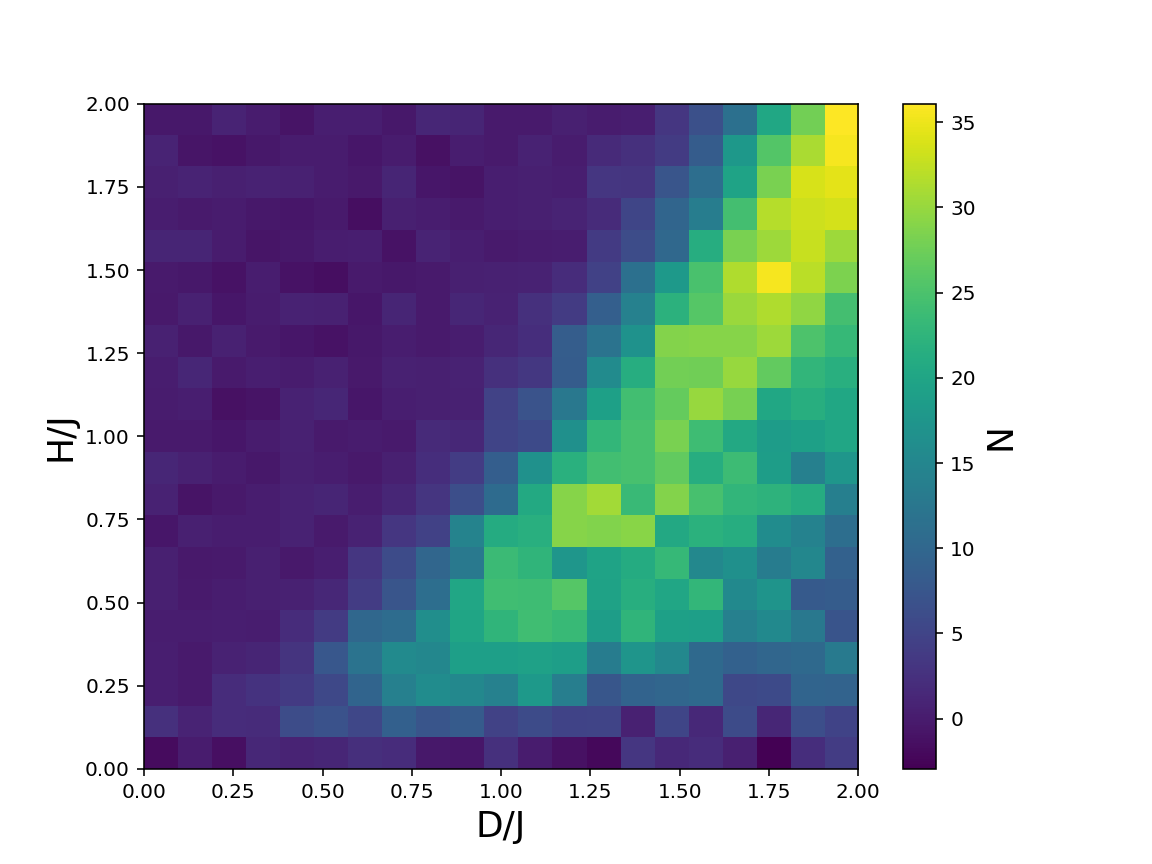
\includegraphics[width=\linewidth]{sections/Graphs/HD_B4.0_NN.png}
%	\caption{The number of detected skyrmions as a function of unitless DM-interaction strength (D) and the unitless applied magnetic field (H).}
%\end{figure}
%
%In the spiral phase there will be many structures that have a wrapping number. These are detected by the algorithm. To separate the spiral phase from the Skyrmionic phase, the the strength of the positive wrapping and negative wrapping are tracked. If the positive and negative wrapping are about as strong there is a spiral phase, while if the negative is much larger than the positive there are Skyrmions. Here the skyrmionic phase is then selected to be the domain where the negative peak hight is 1.5 times greater then the positive peak hight. This domain is shown in figure \ref{}.
%
%\begin{figure}[H]
%	\centering
%	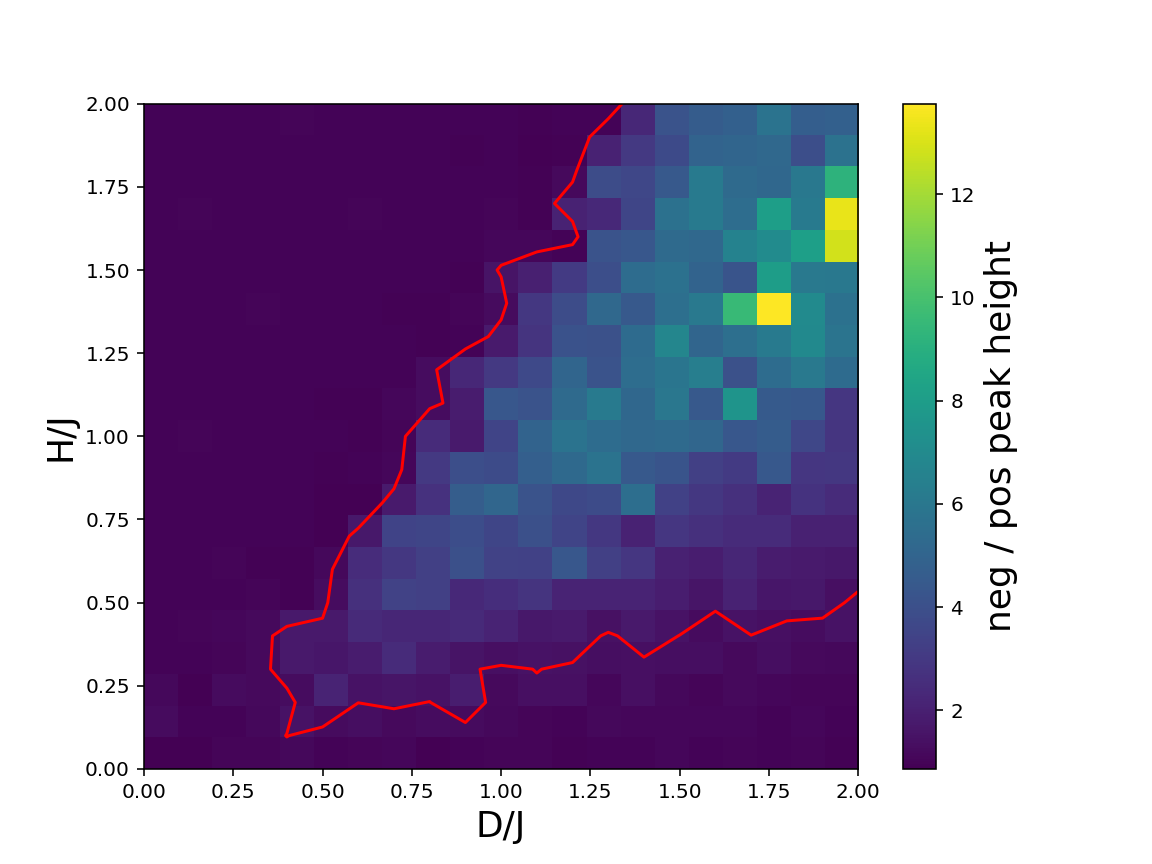
\includegraphics[width=\linewidth]{sections/Graphs/HD_B4.0_PH_NH.png}
%	\caption{The detected hight of the negative detected skyrmions divided by the hight of the positive detected skyrmion as a function of unitless DM-interaction strength (D) and the unitless applied magnetic field (H).}
%\end{figure}
%
%To separate the spiral phase from the ferromagnetic phase from the spyral phase the average magnetization pointing along the direction of the magnetic field can be calculated as shown in figure \ref{}. We know that for the spiral phase there shouldn't be a strong preference for the spin pointing up or down sinse the DM onteraction domminates.
%
%\begin{figure}[H]
%	\centering
%	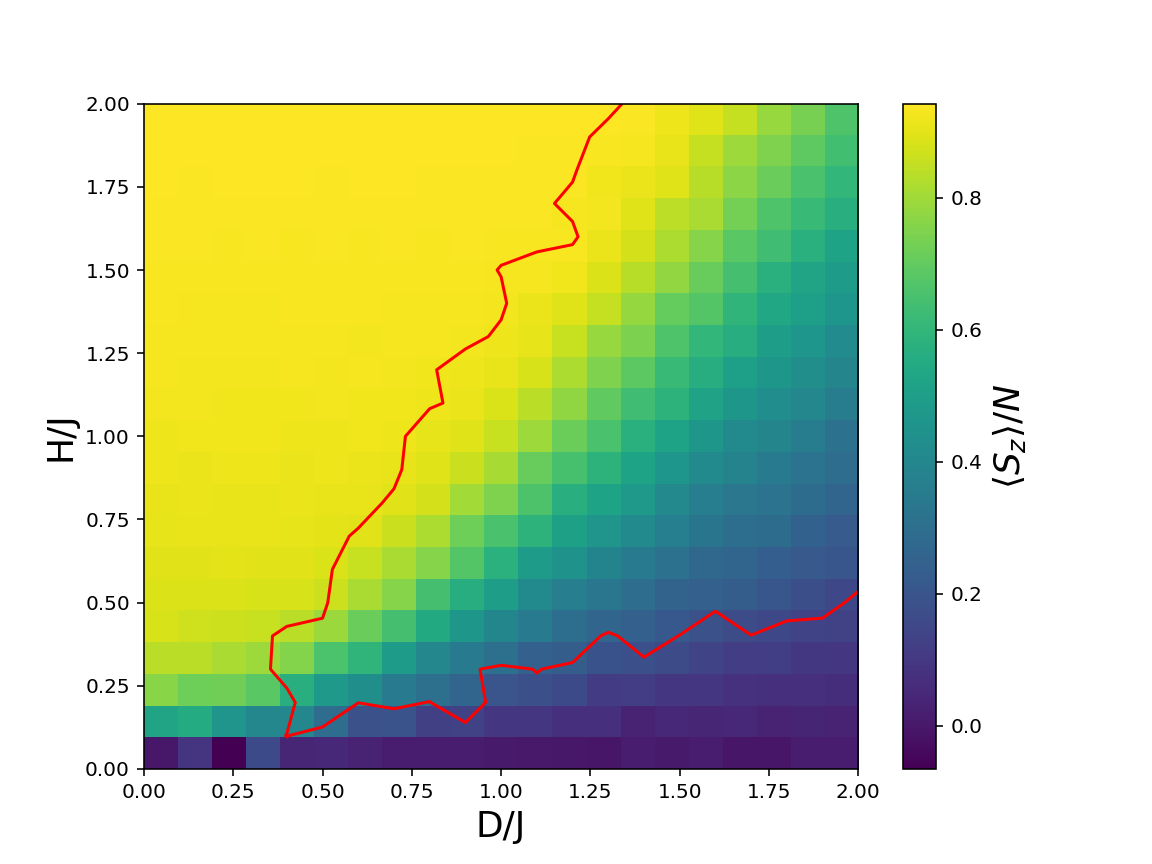
\includegraphics[width=\linewidth]{sections/Graphs/HD_B4.0_AM.png}
%	\caption{The average magnetization in the Z direction as a function of unitless DM-interaction strength (D) and the unitless applied magnetic field (H).}
%\end{figure}
%

\subsection{Distinguishing phases}

Three distinct phases are observed in the simulations: a ferromagnetic phase, a spiral phase, and a skyrmionic phase. To determine which phase is present for a given combination of DM interaction strength and applied magnetic field, several observables are evaluated.

The phase diagram is constructed by varying the dimensionless DM interaction strength (D) and the dimensionless magnetic field (H), while keeping the exchange interaction constant. For each parameter combination, the skyrmion detection algorithm described in the previous section is applied. The resulting number of detected skyrmions is shown in Figure~\ref{fig: skyrmion_count}.

\begin{figure}[H]
	\centering
	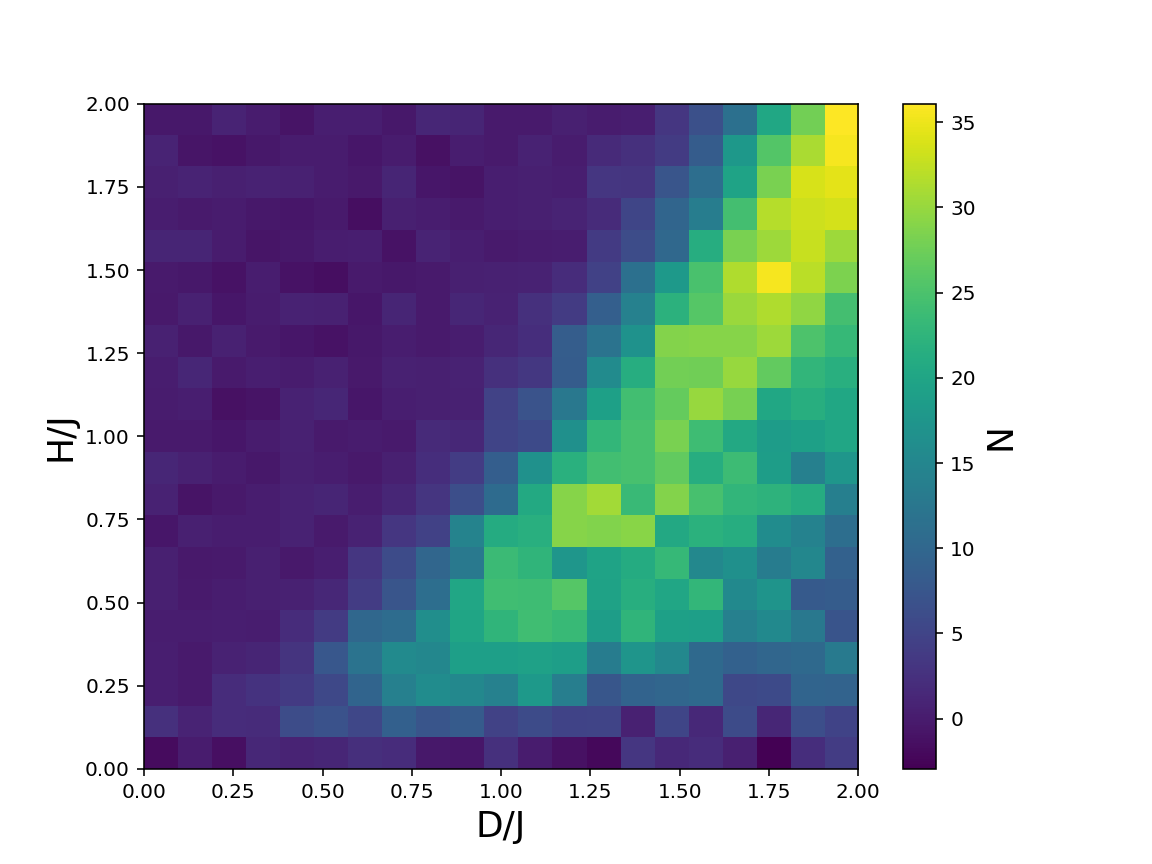
\includegraphics[width=\linewidth]{sections/Graphs/HD_B4.0_NN.png}
	\caption{The number of detected skyrmions as a function of the dimensionless DM interaction strength (D) and the dimensionless applied magnetic field (H).}
	\label{fig: skyrmion_count}
\end{figure}

The number of detected skyrmions alone is not sufficient to distinguish the skyrmionic phase from the spiral phase. In the spiral phase, extended spin textures can also generate localized extrema in the topological charge density, causing the detection algorithm to identify structures that are not isolated skyrmions.

To separate these phases, the relative magnitudes of the positive and negative extrema in the smoothed topological charge density are considered. In the spiral phase, positive and negative extrema occur with comparable magnitude, reflecting the absence of isolated topological objects. In contrast, the skyrmionic phase is characterized by strong negative peaks associated with skyrmion cores and significantly weaker positive peaks. Figure~\ref{fig: wrapping_ratio} shows the ratio between the magnitudes of the negative and positive extrema.

The skyrmionic phase is defined as the region where the average magnitude of the negative extrema exceeds that of the positive extrema by a factor of at least 1.5.

\begin{figure}[H]
	\centering
	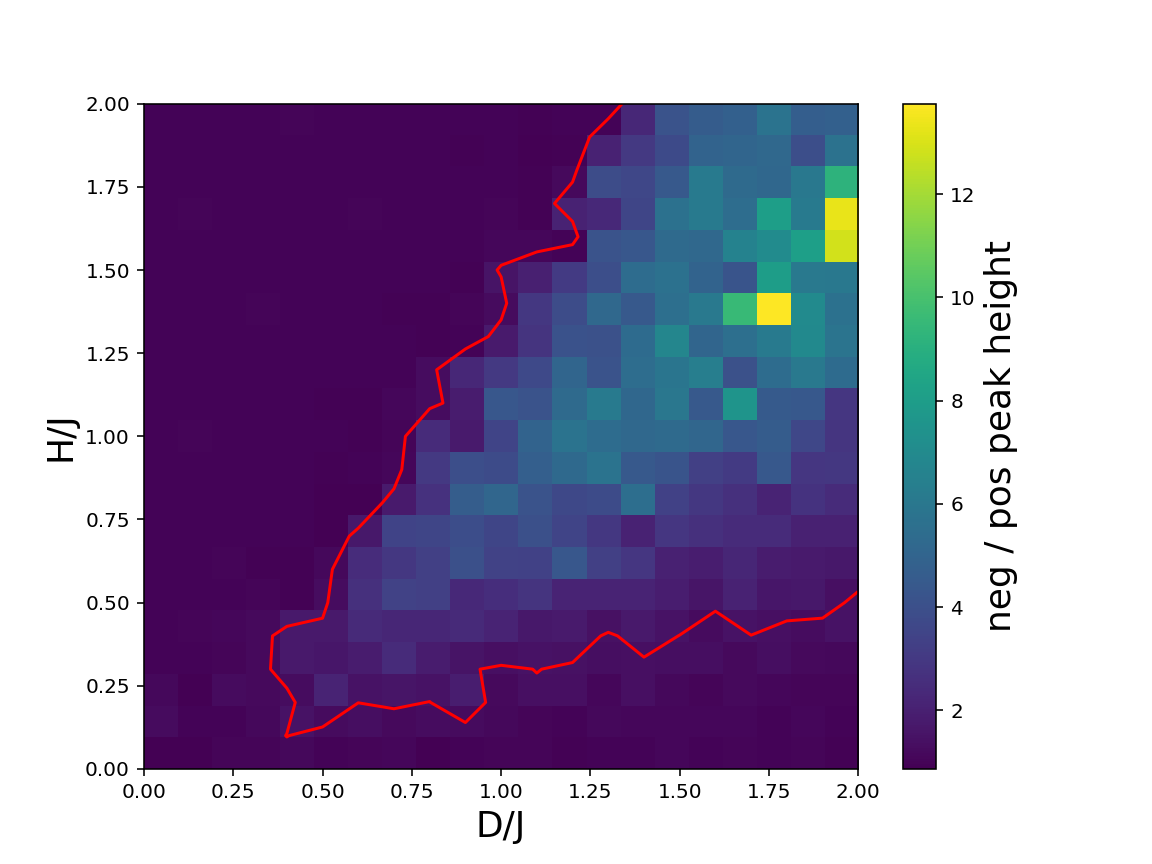
\includegraphics[width=\linewidth]{sections/Graphs/HD_B4.0_PH_NH.png}
	\caption{Ratio between the magnitudes of the detected negative and positive extrema in the smoothed topological charge density as a function of the dimensionless DM interaction strength (D/J) and the dimensionless applied magnetic field (H/J).}
	\label{fig: wrapping_ratio}
\end{figure}

The ferromagnetic and spiral phases are distinguished using the average magnetization along the direction of the applied magnetic field.
In the ferromagnetic phase, the Zeeman interaction dominates and most spins align with the magnetic field. In the spiral phase, the DM interaction dominates and the spins preferentially lie in the (xy)-plane, giving a much smaller value of  the average magnetization. The resulting average magnetization is shown in Figure~\ref{fig: magnetization_phase}.

\begin{figure}[H]
	\centering
	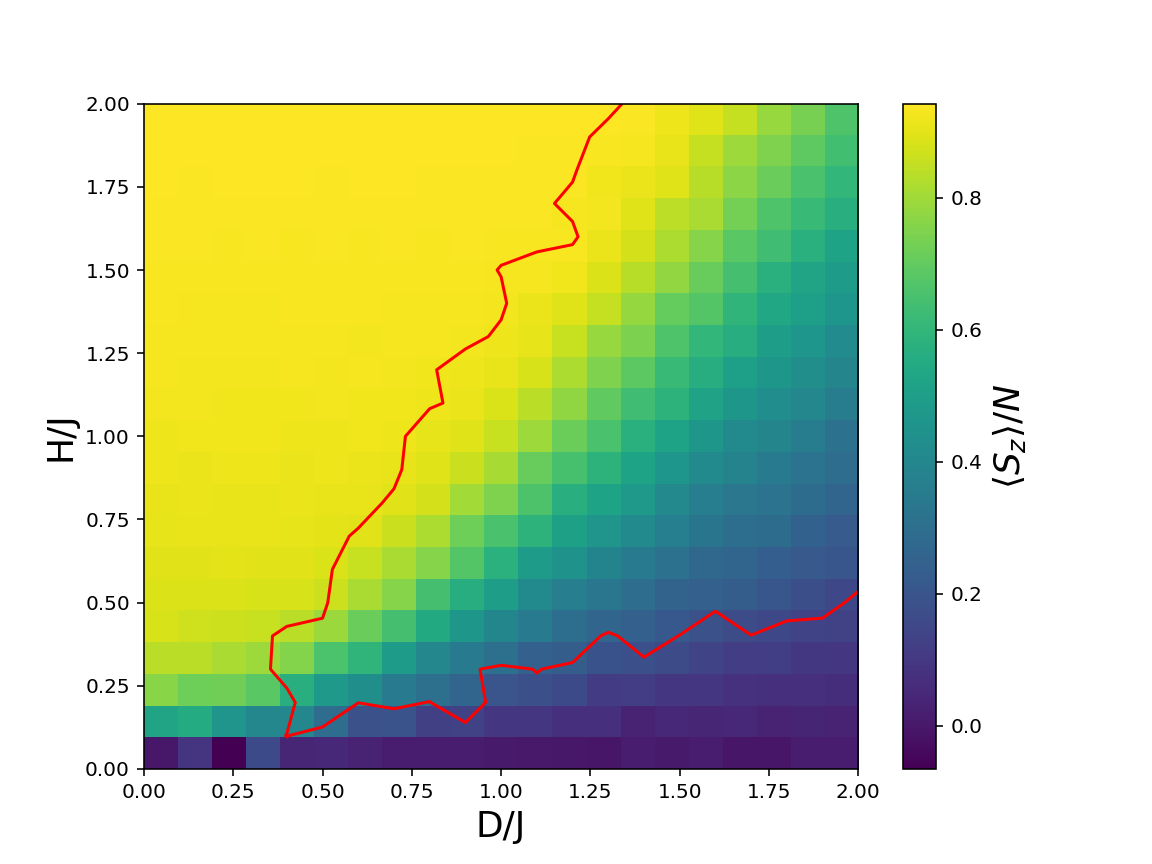
\includegraphics[width=\linewidth]{sections/Graphs/HD_B4.0_AM.png}
	\caption{Average magnetization in the direction of the applied magnetic field as a function of the dimensionless DM interaction strength (D/J) and the dimensionless applied magnetic field (H/J). Also indicated is the domain where skyrmions are found (red).}
	\label{fig: magnetization_phase}
\end{figure}

Combining the skyrmion detection results, the extrema ratio, and the average magnetization allows the ferromagnetic, spiral, and skyrmionic phases to be identified throughout the (D,H) parameter space.


%\subsection{Different Temperatures}
%
%For a better understanding of the circumstances of skyrmion formation occurs the simulation has been repeated for multiple temperatures. To better understand the circumstances of skyrmion destruction simulations have been done that go to $\beta/J = 4$ to a $\beta/J = 0.25$ to see where the skyrmions break down.
%
%\subsubsection{Formation}
%
%To better understand the behavior of skyrmion creation the simulation has been done for multiple temperatures for all combinations of H/J and D/J studied, to see how many skyrmions are formed as a function of temperature. Figure~\ref{fig: Formation} shows how with increasing temperatures less and less skyrmions are formed. The cutoff temperature ($T_f^*$) is decided by when the detected skyrmions reach 30\% of its original count at $\beta/J=4$.
%
%
%\begin{figure}[H]
%	\centering
%	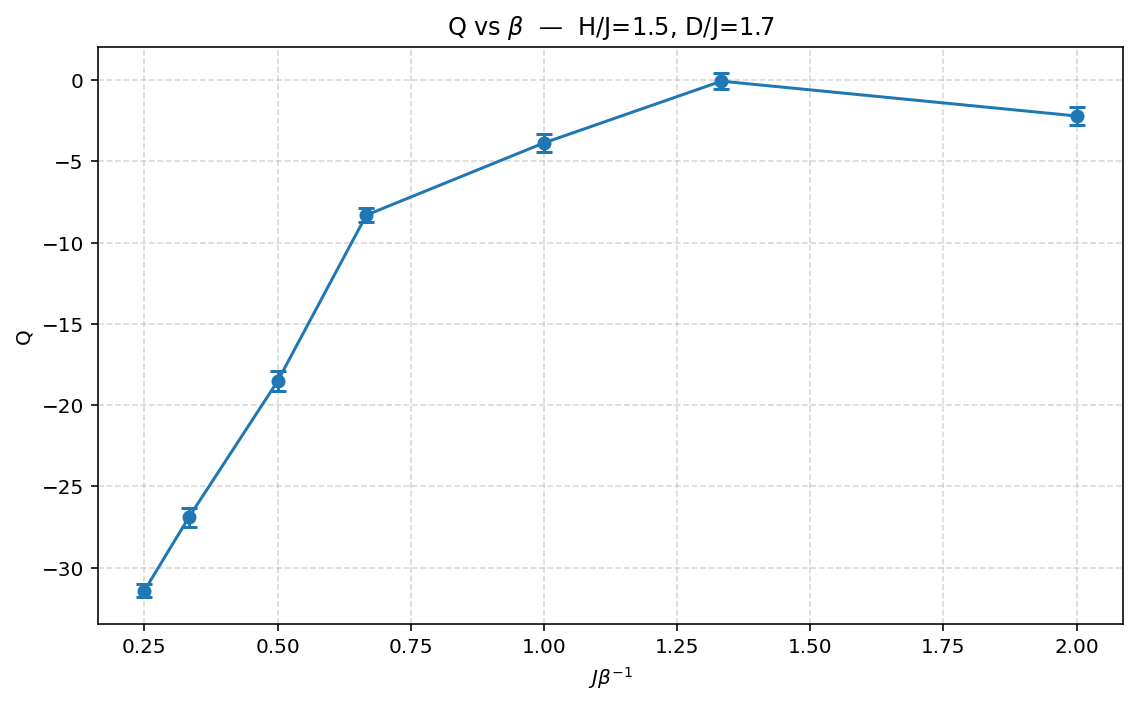
\includegraphics[width=\linewidth]{sections/Graphs/QB1.png}
%	\caption{The detected number of formed skyrmions as a function of unitless temperature for a specific unitless DM-interaction strength (D/J) and the unitless applied magnetic field (H/J).}
%	\label{fig: Formation}
%\end{figure}
%
%
%
%\begin{figure}[H]
%	\centering
%	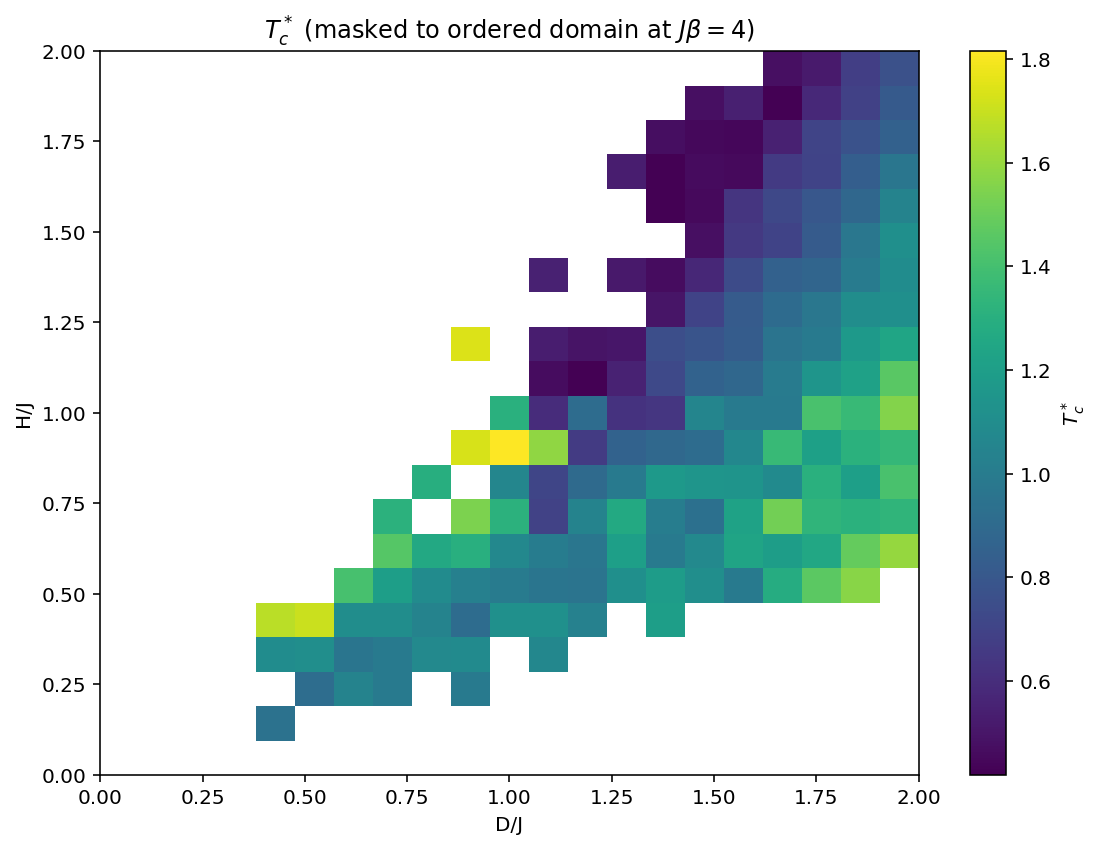
\includegraphics[width=\linewidth]{sections/Graphs/Tf.png}
%	\caption{The formation cutoff temperature as a function of unitless DM-interaction strength (D/J) and the unitless applied magnetic field (H/J).}
%	\label{fig: Formation whole domain}
%\end{figure}
%
%
%\subsubsection{Destruction}
%
%\begin{figure}[H]
%	\centering
%	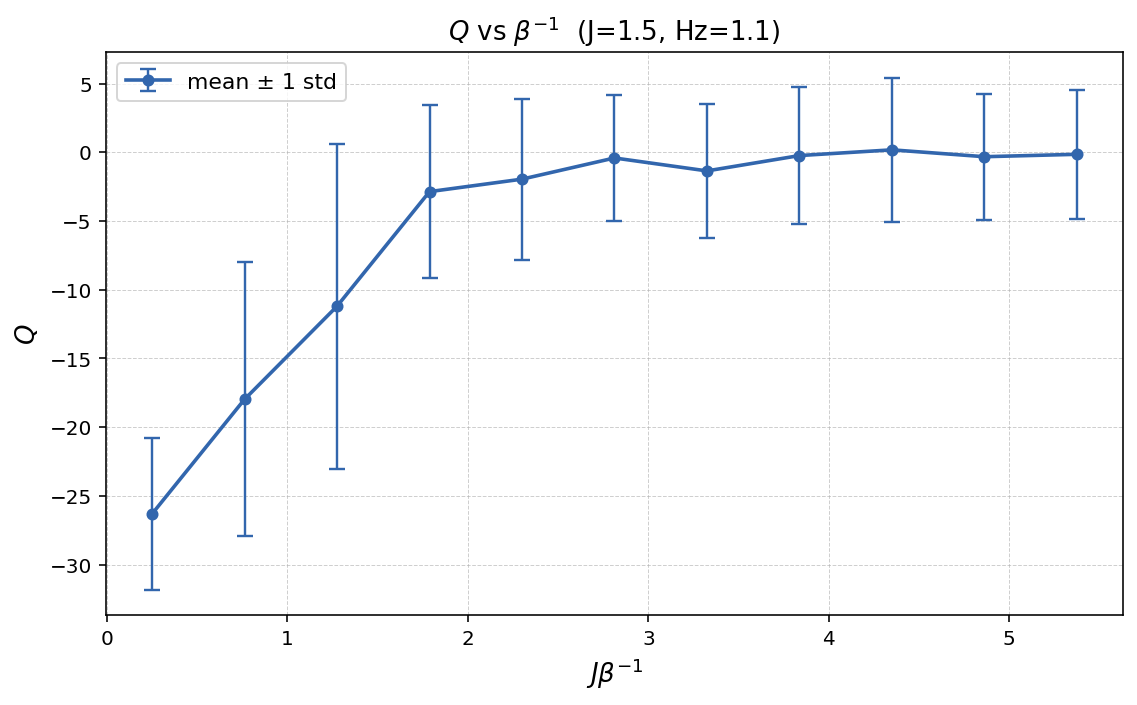
\includegraphics[width=\linewidth]{sections/Graphs/QT.png}
%	\caption{The detected number of existing skyrmions as a function of unitless temperature for a specific unitless DM-interaction strength (D) and the unitless applied magnetic field (H).}
%\end{figure}
%
%\begin{figure}[H]
%	\centering
%	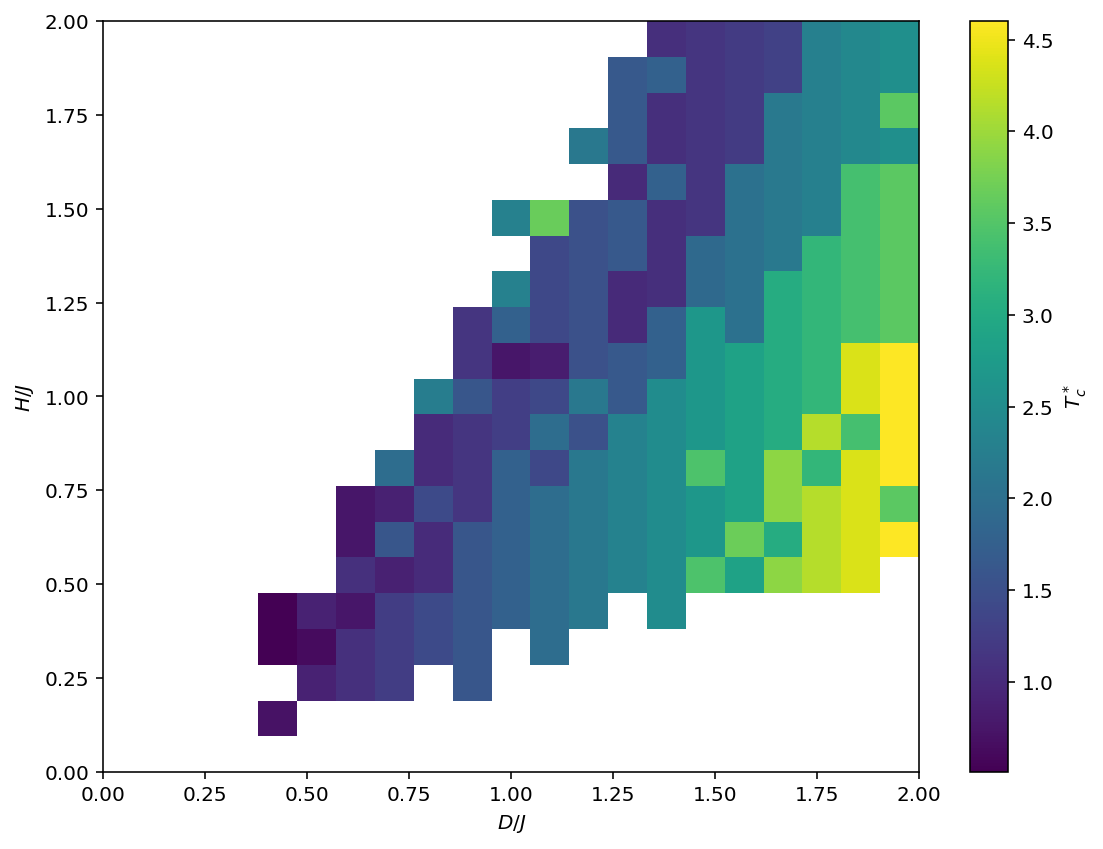
\includegraphics[width=\linewidth]{sections/Graphs/Tc2.png}
%	\caption{The destruction cutoff temperature as a function of unitless DM-interaction strength (D) and the unitless applied magnetic field (H).}
%\end{figure}
\subsection{Formation}

For each combination of \(D/J\) and \(H/J\), the system is initialised at low temperature and gradually heated. The global skyrmion number is recorded as a function of temperature. Figure~\ref{fig: Formation} shows an example where the skyrmion number decreases with increasing temperature due to thermal fluctuations destabilising the topological textures.

\begin{figure}[H]
	\centering
	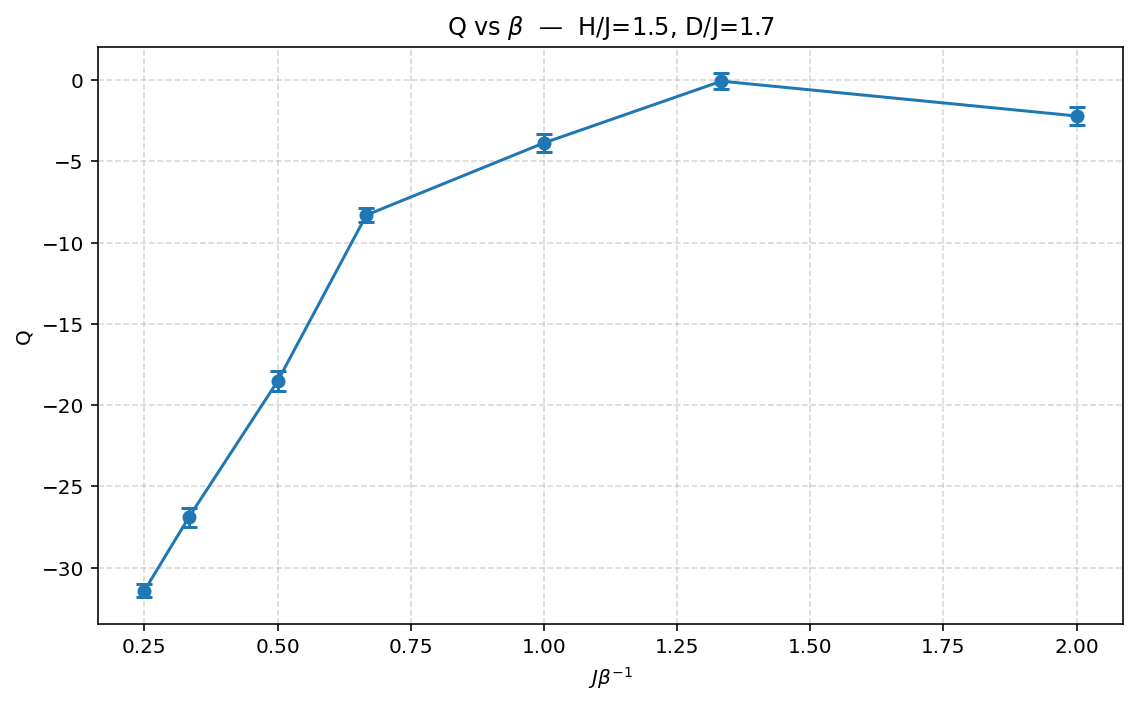
\includegraphics[width=\linewidth]{sections/Graphs/QB1.png}
	\caption{Number of formed skyrmions as a function of dimensionless temperature for fixed values of \(D/J\) and \(H/J\).}
	\label{fig: Formation}
\end{figure}

The formation cutoff temperature \(T_f^*\) is defined in context of
\begin{equation}
	Q=a+b e^{-\frac{J\beta^{-1}}{T_f^*}}.
\end{equation}
This equation is fit to the data to get the cutoff temperature.
The resulting dependence on \(D/J\) and \(H/J\) is shown in Figure~\ref{fig: Formation whole domain}.

\begin{figure}[H]
	\centering
	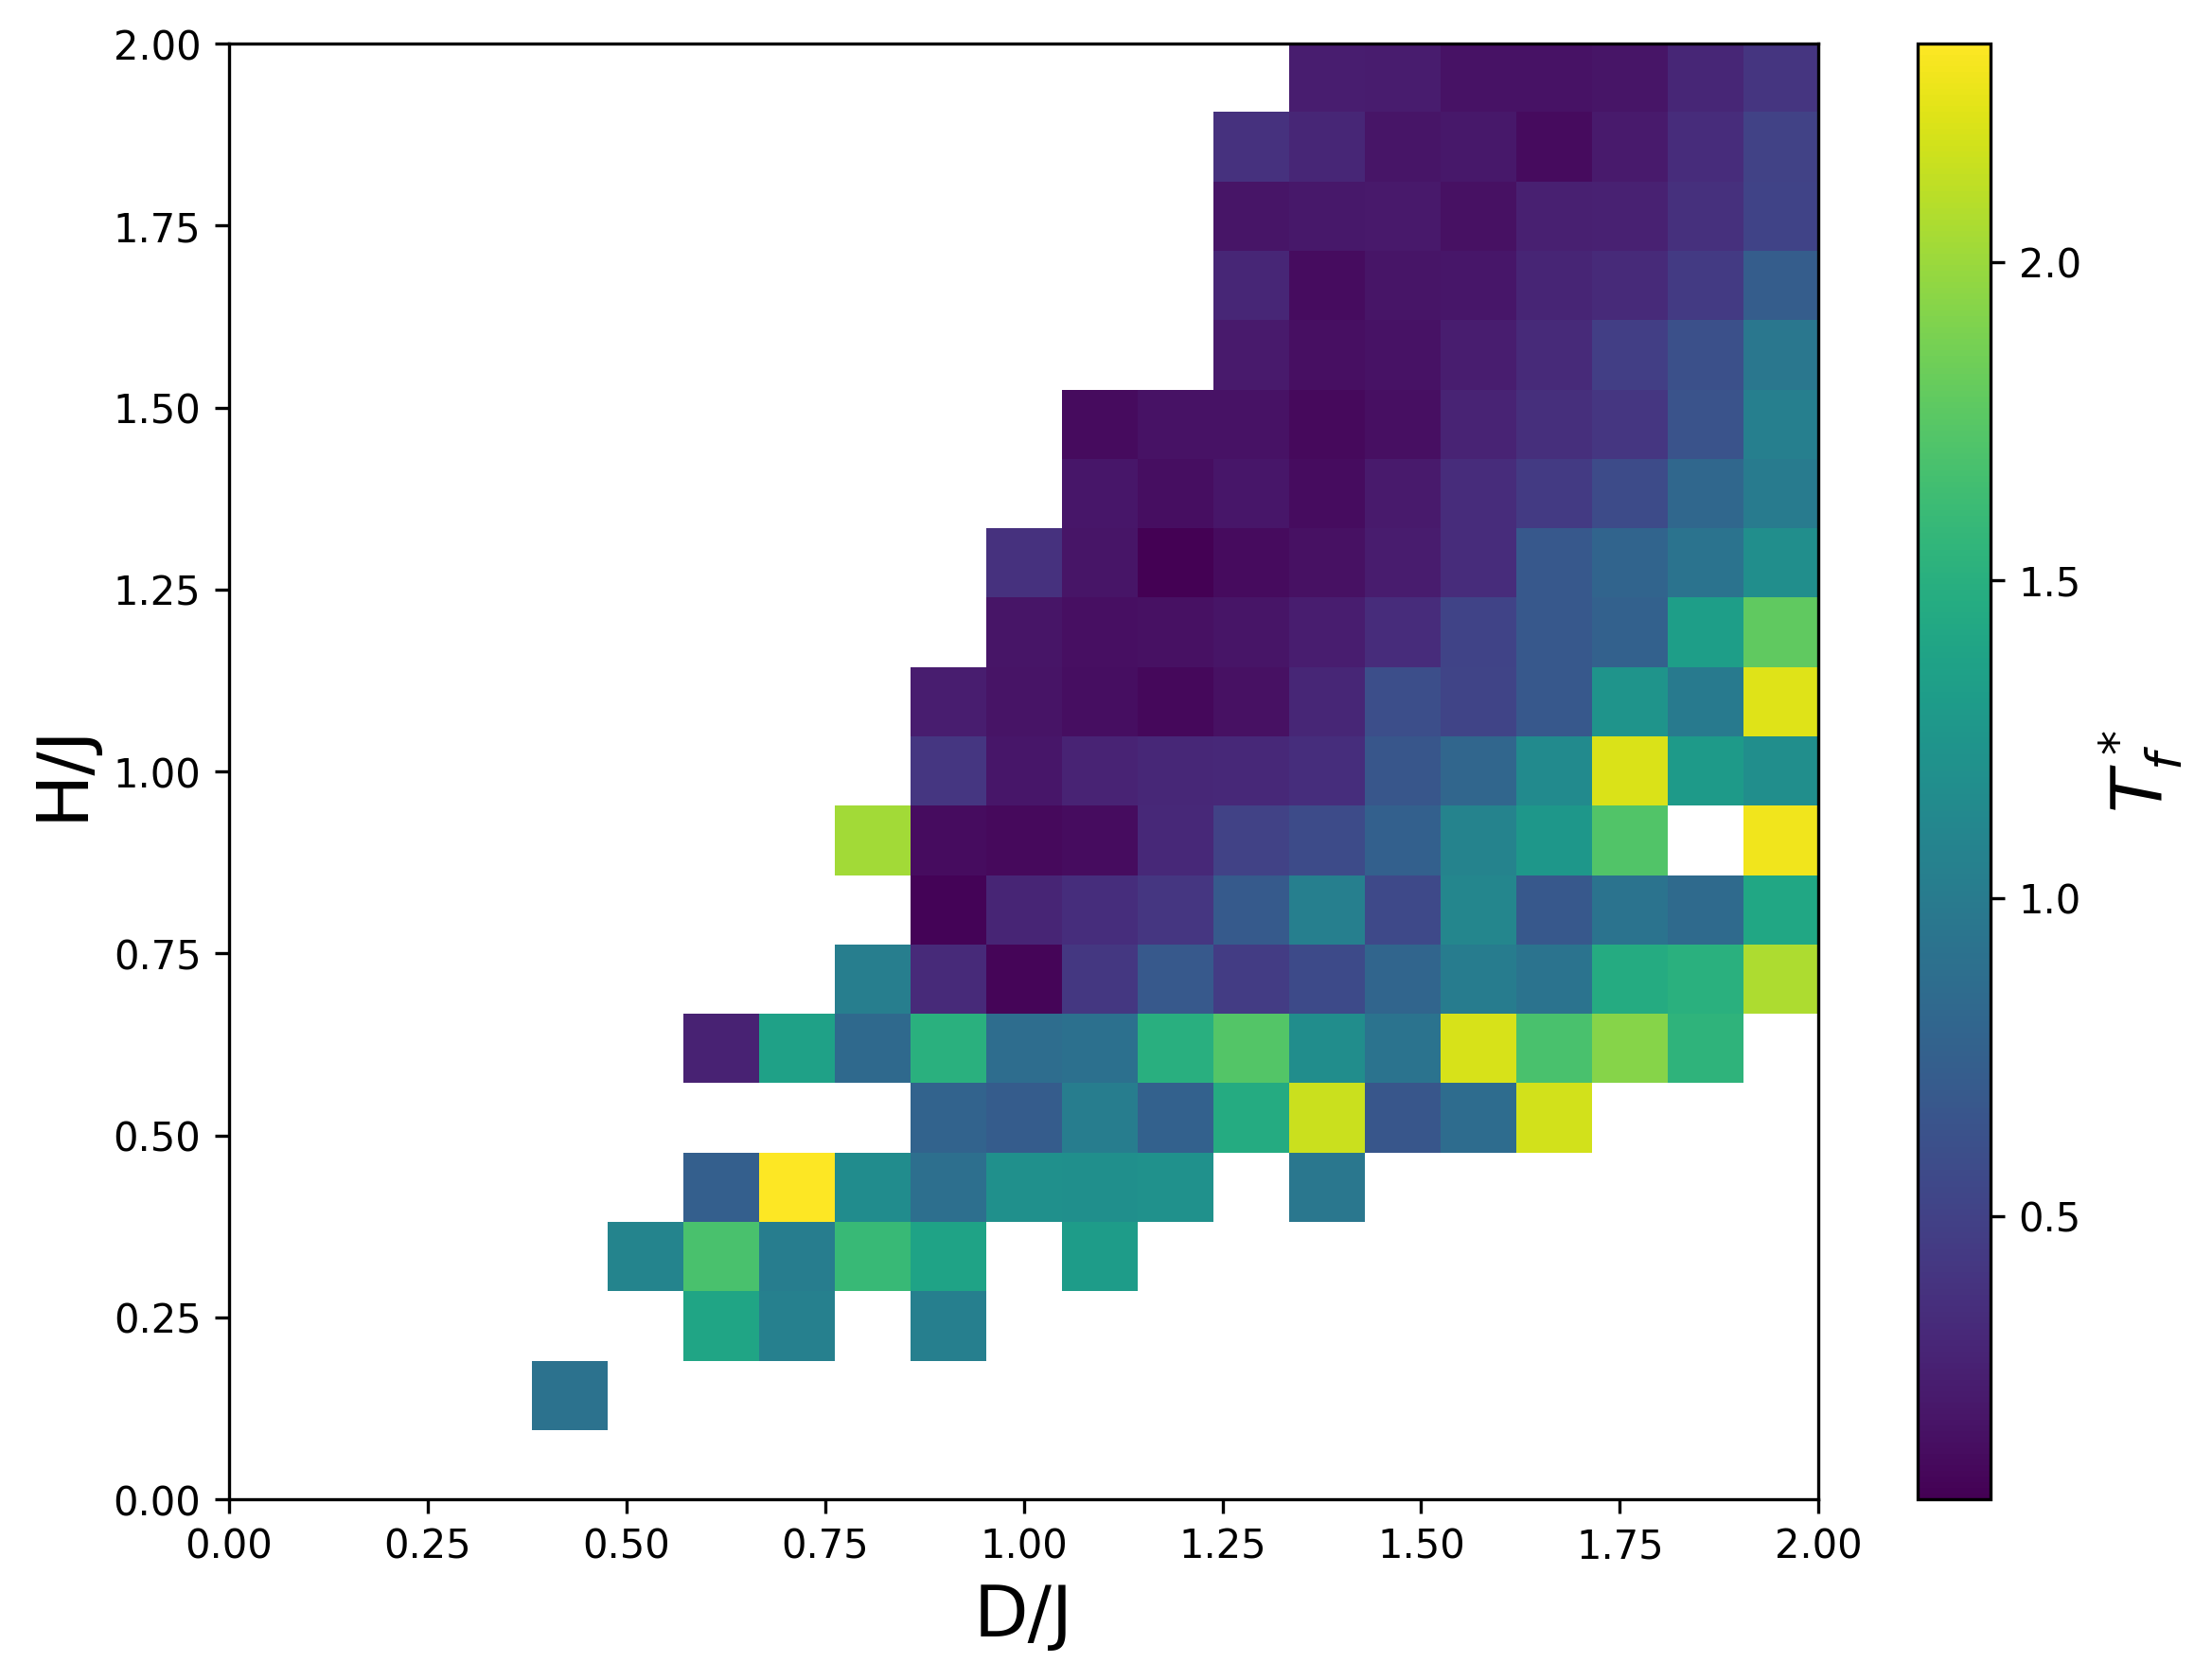
\includegraphics[width=\linewidth]{sections/Graphs/Tf_masked.png}
	\caption{Formation cutoff temperature \(T_f^*\) as a function of dimensionless DM interaction strength \(D/J\) and applied magnetic field \(H/J\).}
	\label{fig: Formation whole domain}
\end{figure}


\subsection{Destruction}

In this case, the system is initialised in a low-temperature skyrmionic configuration and subsequently heated. The number of surviving skyrmions is tracked as a function of temperature, as shown in Figure~\ref{fig: QT}. At sufficiently high temperature, thermal fluctuations destroy the skyrmionic textures and the detected skyrmion number approaches zero.

\begin{figure}[H]
	\centering
	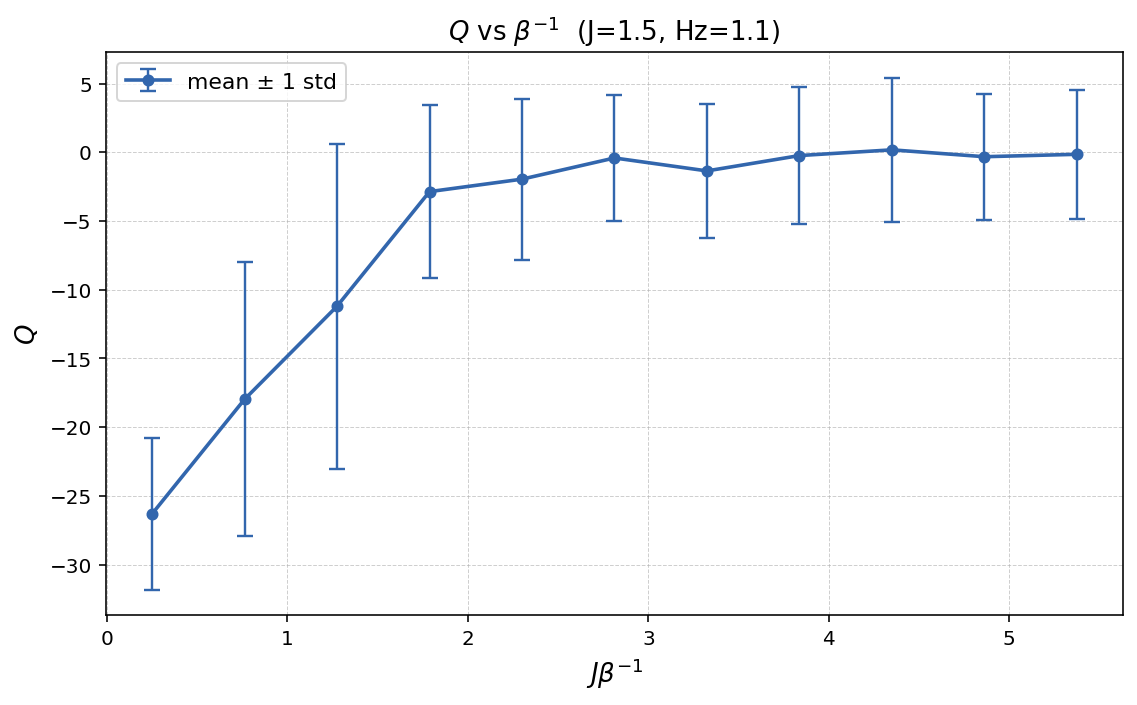
\includegraphics[width=\linewidth]{sections/Graphs/QT.png}
	\caption{Number of surviving skyrmions as a function of dimensionless temperature for fixed values of \(D/J\) and \(H/J\).}
	\label{fig: QT}
\end{figure}

The destruction cutoff temperature \(T_c^*\) is defined in context of
\begin{equation}
	Q=a+b e^{-\frac{J\beta^{-1}}{T_c^*}}.
\end{equation}
This equation is fit to the data to get the cutoff temperature.
The resulting dependence on \(D/J\) and \(H/J\) is shown in Figure~\ref{fig: Tc}.

\begin{figure}[H]
	\centering
	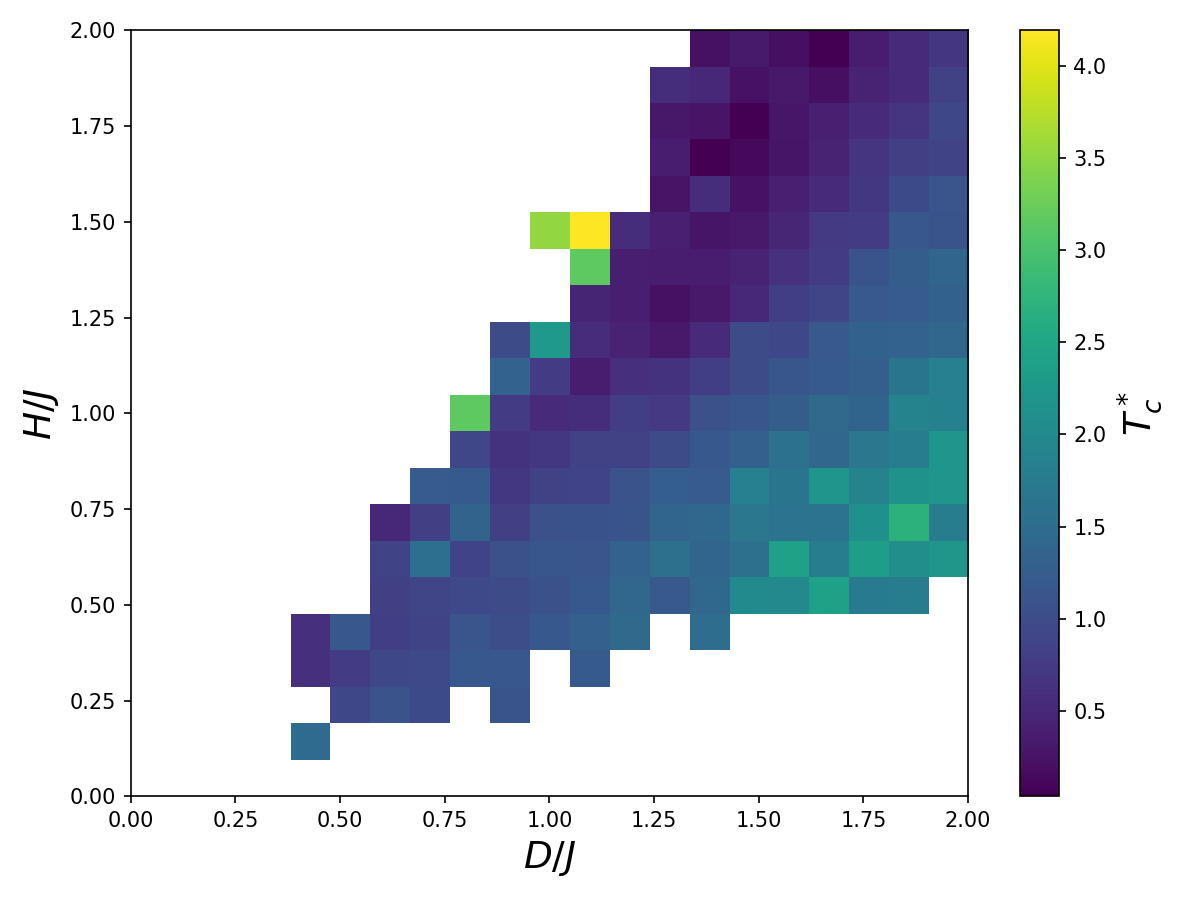
\includegraphics[width=\linewidth]{sections/Graphs/tau_masked.png}
	\caption{Destruction cutoff temperature \(T_c^*\) as a function of dimensionless DM interaction strength \(D/J\) and applied magnetic field \(H/J\).}
	\label{fig: Tc}
\end{figure}
